\section{eo\-General\-Real\-Bounds Class Reference}
\label{classeo_general_real_bounds}\index{eoGeneralRealBounds@{eoGeneralRealBounds}}
A class that encapsulate all possible {\bf eo\-Int\-Bounds}{\rm (p.\,\pageref{classeo_int_bounds})}.  


{\tt \#include $<$eo\-Real\-Bounds.h$>$}

Inheritance diagram for eo\-General\-Real\-Bounds::\begin{figure}[H]
\begin{center}
\leavevmode
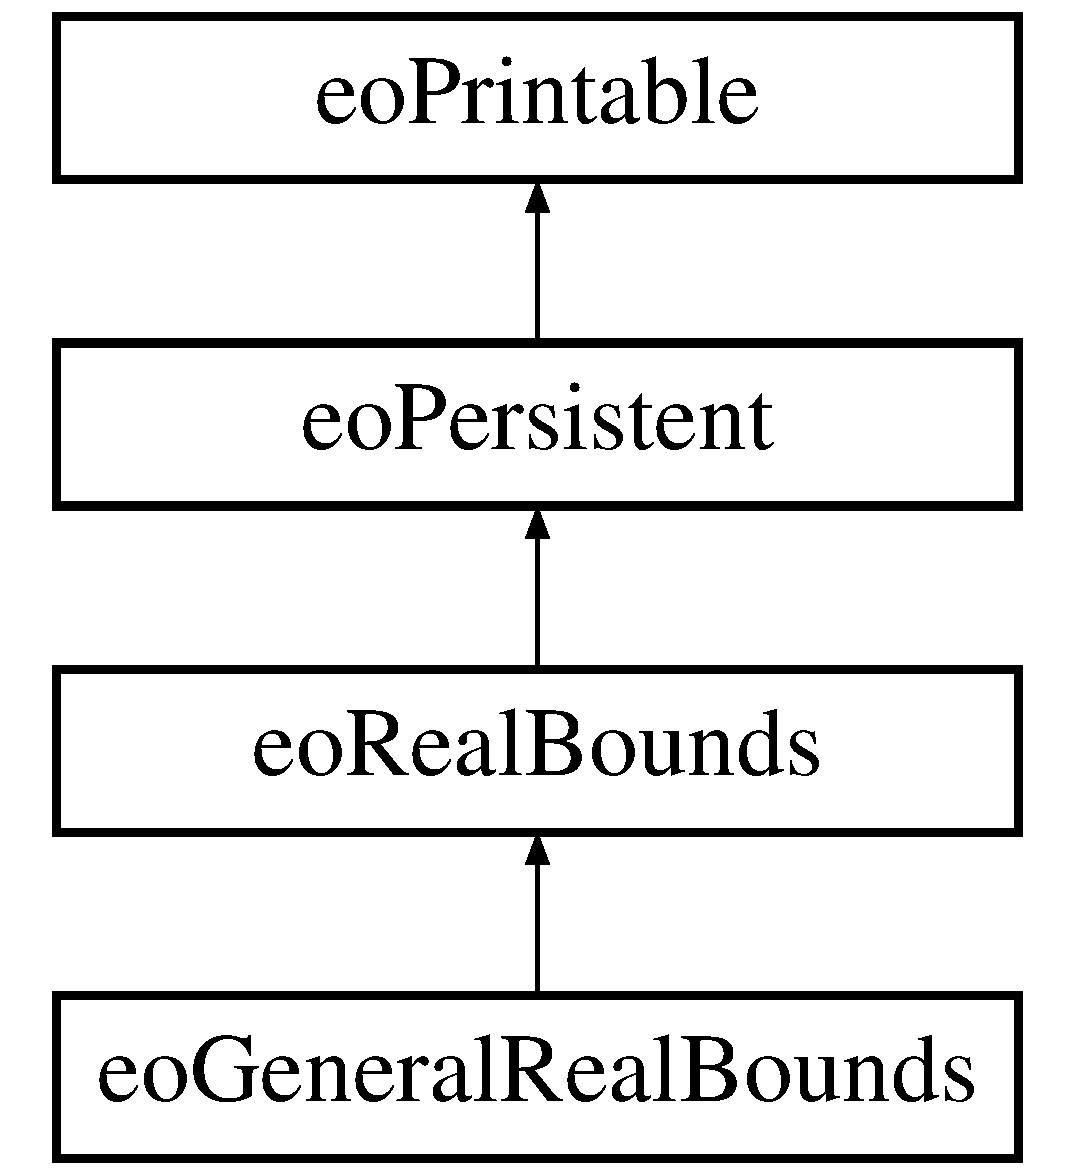
\includegraphics[height=4cm]{classeo_general_real_bounds}
\end{center}
\end{figure}
\subsection*{Public Member Functions}
\begin{CompactItemize}
\item 
{\bf eo\-General\-Real\-Bounds} (std::string \_\-s=\char`\"{}[-infinity,+infinity]\char`\"{})\label{classeo_general_real_bounds_a0}

\begin{CompactList}\small\item\em Ctor: from a string, chooses the type of bound. \item\end{CompactList}\item 
{\bf eo\-General\-Real\-Bounds} (const {\bf eo\-General\-Real\-Bounds} \&\_\-b)\label{classeo_general_real_bounds_a1}

\begin{CompactList}\small\item\em Need a Cpy Ctor because we are allocating memory. \item\end{CompactList}\item 
{\bf eo\-General\-Real\-Bounds} \& {\bf operator=} (const {\bf eo\-General\-Real\-Bounds} \&\_\-b)\label{classeo_general_real_bounds_a2}

\item 
{\bf $\sim$eo\-General\-Real\-Bounds} ()\label{classeo_general_real_bounds_a3}

\begin{CompactList}\small\item\em Need a Dtor because we allocate an actual bound. \item\end{CompactList}\item 
virtual bool {\bf is\-Bounded} (void) const \label{classeo_general_real_bounds_a4}

\begin{CompactList}\small\item\em Self-Test: true if $\ast$$\ast$$\ast$both$\ast$$\ast$$\ast$ a min and a max. \item\end{CompactList}\item 
virtual bool {\bf has\-No\-Bound\-At\-All} (void) const \label{classeo_general_real_bounds_a5}

\begin{CompactList}\small\item\em Self-Test: true if no min $\ast$$\ast$$\ast$and$\ast$$\ast$$\ast$ no max hence no further need to test/truncate/fold anything. \item\end{CompactList}\item 
virtual bool {\bf is\-Min\-Bounded} (void) const \label{classeo_general_real_bounds_a6}

\begin{CompactList}\small\item\em Self-Test: bounded from below??? \item\end{CompactList}\item 
virtual bool {\bf is\-Max\-Bounded} (void) const \label{classeo_general_real_bounds_a7}

\begin{CompactList}\small\item\em Self-Test: bounded from above??? \item\end{CompactList}\item 
virtual bool {\bf is\-In\-Bounds} (double \_\-x) const \label{classeo_general_real_bounds_a8}

\begin{CompactList}\small\item\em Test on a value: is it in bounds? \item\end{CompactList}\item 
virtual void {\bf folds\-In\-Bounds} (double \&\_\-x) const \label{classeo_general_real_bounds_a9}

\begin{CompactList}\small\item\em Put value back into bounds - by folding back and forth. \item\end{CompactList}\item 
virtual void {\bf truncate} (double \&\_\-x) const \label{classeo_general_real_bounds_a10}

\begin{CompactList}\small\item\em Put value back into bounds - by truncating to a boundary value. \item\end{CompactList}\item 
virtual double {\bf minimum} () const \label{classeo_general_real_bounds_a11}

\begin{CompactList}\small\item\em get minimum value ::exception if does not exist \item\end{CompactList}\item 
virtual double {\bf maximum} () const \label{classeo_general_real_bounds_a12}

\begin{CompactList}\small\item\em get maximum value ::exception if does not exist \item\end{CompactList}\item 
virtual double {\bf range} () const \label{classeo_general_real_bounds_a13}

\begin{CompactList}\small\item\em get range ::exception if unbounded \item\end{CompactList}\item 
virtual double {\bf uniform} ({\bf eo\-Rng} \&\_\-rng=eo::rng) const \label{classeo_general_real_bounds_a14}

\begin{CompactList}\small\item\em random generator of uniform numbers in bounds ::exception if unbounded \item\end{CompactList}\item 
virtual {\bf eo\-Real\-Bounds} $\ast$ {\bf dup} () const \label{classeo_general_real_bounds_a15}

\begin{CompactList}\small\item\em for memory managements - ugly \item\end{CompactList}\item 
const {\bf eo\-Real\-Bounds} \& {\bf the\-Bounds} () const \label{classeo_general_real_bounds_a16}

\begin{CompactList}\small\item\em for efficiency, it's better to use the embedded boud directly \item\end{CompactList}\item 
virtual void {\bf print\-On} (std::ostream \&\_\-os) const \label{classeo_general_real_bounds_a17}

\begin{CompactList}\small\item\em don't forget the print\-On method - again that of the embedded bound \item\end{CompactList}\item 
virtual void {\bf read\-From} (std::istream \&\_\-is)\label{classeo_general_real_bounds_a18}

\begin{CompactList}\small\item\em no read\-From ??? Have to check that later \item\end{CompactList}\end{CompactItemize}
\subsection*{Private Member Functions}
\begin{CompactItemize}
\item 
{\bf eo\-Real\-Bounds} $\ast$ {\bf get\-Bounds\-From\-String} (std::string)\label{classeo_general_real_bounds_d0}

\begin{CompactList}\small\item\em the constructor for eo\-General\-Real\-Bound - from a string very similar to the {\bf eo\-Real\-Vector\-Bounds::read\-From}{\rm (p.\,\pageref{classeo_real_vector_bounds_a7})} above but was written much later so the read\-From does not call this one as it should do \item\end{CompactList}\end{CompactItemize}
\subsection*{Private Attributes}
\begin{CompactItemize}
\item 
{\bf eo\-Real\-Bounds} $\ast$ {\bf rep\-Bound}\label{classeo_general_real_bounds_r0}

\end{CompactItemize}


\subsection{Detailed Description}
A class that encapsulate all possible {\bf eo\-Int\-Bounds}{\rm (p.\,\pageref{classeo_int_bounds})}. 

Mandatory in order to read through the parser 



Definition at line 506 of file eo\-Real\-Bounds.h.

The documentation for this class was generated from the following files:\begin{CompactItemize}
\item 
eo\-Real\-Bounds.h\item 
eo\-Real\-Bounds.cpp\end{CompactItemize}
